\documentclass{standalone}
\usepackage{pgfplots}

\usepackage{mathtools}
\pgfplotsset{compat=1.8}

% interpolació per a l'exercici/problema pro_interpolacio.tex aparegut a l'examen del segon parcial de mates. Gener 2022

% polinomi obtingut amb el codi polinomisBeziers.mlx

\begin{document}

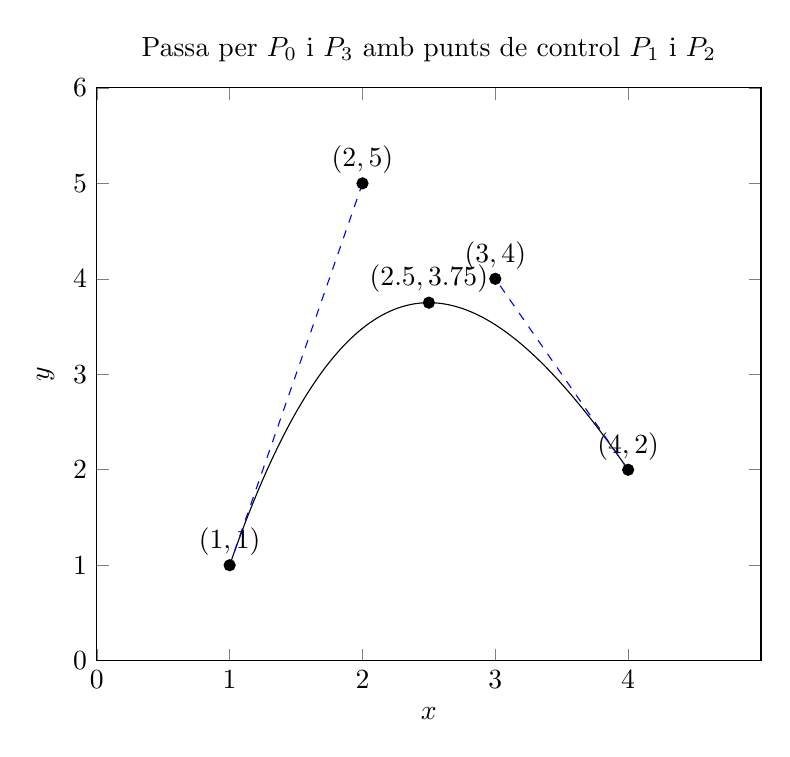
\begin{tikzpicture}
\pgfplotsset{
  scale only axis,
  xmin=0,xmax=5,
  ymin=0,ymax=6,
  xlabel=$x$,
  ylabel=$y$,
  samples=100,
  xtick={0,1,2,3,4}
%  yticklabel style={text width=3em,align=right}% important per mantenir una mida correcta dels ticks en qualsevol situació quan hi ha multiple plots
}

\begin{axis}[
  title={Passa per $P_0$ i $P_3$ amb punts de control $P_1$ i $P_2$},
  %name=plot2,
  %at=(plot1.right of south east), anchor=left of south west,
  ]
  \addplot [only marks,mark=*,nodes near coords={$(\pgfmathprintnumber{\pgfkeysvalueof{/data point/x}},
   \pgfmathprintnumber{\pgfkeysvalueof{/data point/y}})$}]
   table {
    1 1
    2 5
    3 4
    4 2
    2.5 3.75
    };
  \addplot[][domain=0:1]({3*x+1},{4*x^3-15*x^2+12*x+1});
  \addplot[dashed,blue] coordinates {(4,2) (3,4)};
  \addplot[dashed,blue] coordinates {(2,5) (1,1)};
\end{axis}

\end{tikzpicture}

\end{document}
